\documentclass{if-beamer}
\usepackage{tikz-cd}
\newcommand{\MR}[1]{\href{http://www.ams.org/mathscinet-getitem?mr=#1}{MR#1}}
% --------------------------------------------------- %
%                  Presentation info	              %
% --------------------------------------------------- %
\title[Maximal Function for Semigroup]{On the $L^p$ bound of maximal function for semigroups}
\subtitle{Report for MA545 Topics in Analysis}
\author[Liu]{Xiaoyu Liu} % Add the second author here
\institute[Purdue]{Purdue University \and \textbf{Instructed by Prof. Rodrigos Ba\~nuelos}}


    
\begin{document}

\begin{frame}
  \titlepage
\end{frame}

\section{Motivation}

\begin{frame}{Motivation and goal of the talk}

\begin{block}{Bounds for maximal functions}
    Crucial for
    \begin{itemize}
    \item Lebesgue Differentiation Theorem, approximation to identity
    \item Singular integrals
    \item Fractional integration
    \end{itemize}
    Previous bounds depending on geometry of $\mathbb{R}^n$
    \begin{itemize}
    \item Hardy-Littlewood maximal inequality, via Vitali covering lemma, $C = \left(\frac{2 \cdot 3^n p}{p- 1}\right)^{1/p}$.
    \item Calder\'on-Zygmund theory, via dyadic decomposition, $C = 2^{n/p}$.
    \end{itemize}
\end{block}

\begin{block}{Good to have dimension-free bounds}
    \begin{itemize}
        \item Remove exponential growth in $n$.
        \item Generalizable to manifolds, Lie groups, etc.
    \end{itemize}
\end{block}

\end{frame}

\begin{frame}{Motivation and goal of the talk, cont.}
    The Maximal function for a function $f$ is defined as
    \begin{equation*}
        f^*(x) = \sup_{t > 0} |T_t f(x)|
    \end{equation*}
    With dimension-dependent bounds, we have
    \begin{equation*}
        \left|f^*\right|_p \leq A \left\|Mf\right\|_p \leq A\left(\frac{2 \cdot 3^n p}{p- 1}\right)^{1/p} \left\|f\right\|_p
    \end{equation*}
    \begin{block}{Goal}
        Using probability theory, show
        \begin{equation*}
            \left|f^*\right|_p \leq \frac{p}{p-1} \left\|f\right\|_p
        \end{equation*}
        for all $1<p\leq \infty$.
    \end{block}
\end{frame}

\section{Probablistic Connections}

\begin{frame}{Feller Semigroups and Feller Process}

    \begin{columns}
        \begin{column}{0.5\textwidth}
            \begin{block}{Feller Semigroup}
                A family of operators $P_t$ on $L^p(\mathbb{R}^n)$, $1\leq p\leq \infty$, is a \textbf{Feller semigroup} if
                \begin{itemize}
                    \item $P_t$ is a contraction on $L^p$.
                    \item $P_t$ is \textit{strongly continuous} in $t$.
                    \item $P_t$ is \textit{positivity preserving}.
                \end{itemize}
            \end{block}
            \begin{block}{Feller Process}
                A \textbf{Feller process} is a Markov process with a Feller semigroup.
            \end{block}
            If $P_t$ is self-adjoint on $L^2$, then the process is \textbf{reversible}.
            \begin{exampleblock}{Examples}
                \begin{itemize}
                    \item Heat kernel $\longleftrightarrow$ Brownian motion
                    \item Poisson kernel $\longleftrightarrow$ Cauchy process
                \end{itemize}
            \end{exampleblock}
        \end{column}
        \begin{column}{0.5\textwidth}
            \begin{figure}
                \centering
                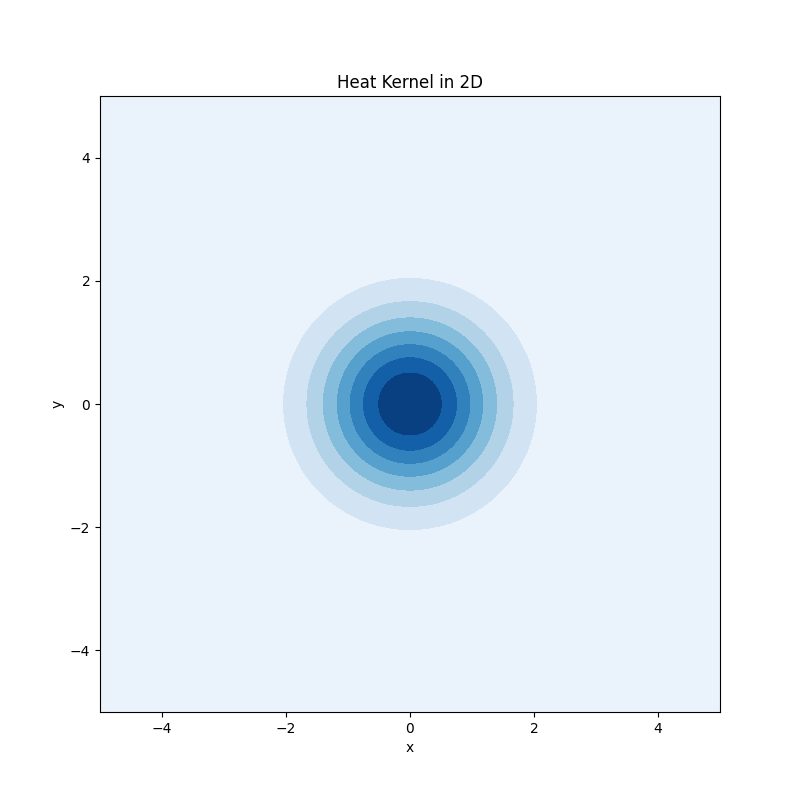
\includegraphics[width=0.5\textwidth]{figures/heat_kernel_2d.png}
            \end{figure}
            \begin{figure}
                \centering
                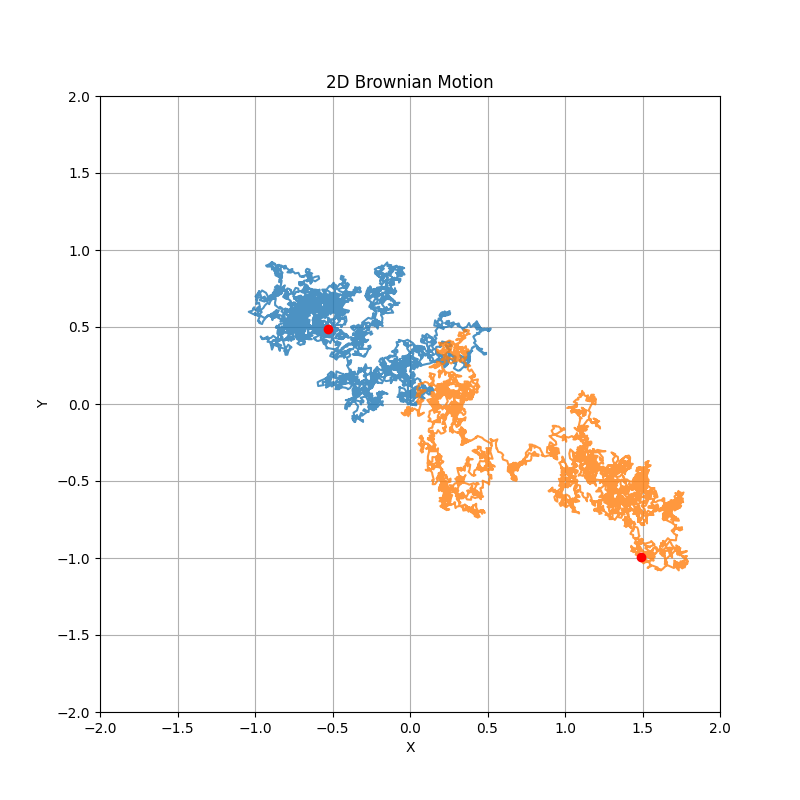
\includegraphics[width=0.5\textwidth]{figures/brownian_motion_2d.png}
            \end{figure}
        \end{column}
    \end{columns}
\end{frame}

\begin{frame}{A physical perspective}
    \begin{columns}
        \begin{column}{0.5\textwidth}
            \begin{block}{Heat semigroup}
                Time-evolution of a diffusion process, irreversible.
            \end{block}
            % space
            \vspace{1em}
            Ensemble Average
            \begin{equation*}
                \frac{1}{N} \sum_{i = 1}^N f(X^{(i)}_t) \xrightarrow{N \to \infty} \mathbb{E}[f(X_t)] = H_t f 
            \end{equation*}

            % space
            \vspace{1em}

            \begin{block}{Brownian Motion}
                Microscopic model of particles in heat motion, reversible.
            \end{block}
            
        \end{column}
        \begin{column}{0.5\textwidth}
            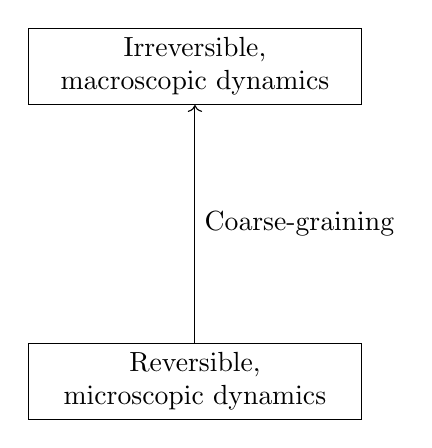
\begin{tikzpicture}
                \node (A) at (0,0) [draw, rectangle, text width=4cm, align=center] {Reversible,\\ microscopic dynamics};
                \node (B) at (0,4) [draw, rectangle, text width=4cm, align=center] {Irreversible,\\ macroscopic dynamics};
                \draw[->] (A) -- (B) node[midway, right] {Coarse-graining};
            \end{tikzpicture}
            
            
        \end{column}
    \end{columns}
\end{frame}

\begin{frame}{A physical perspective, cont.}
    \begin{columns}
        \begin{column}{0.5\textwidth}
            \begin{figure}
                \centering
                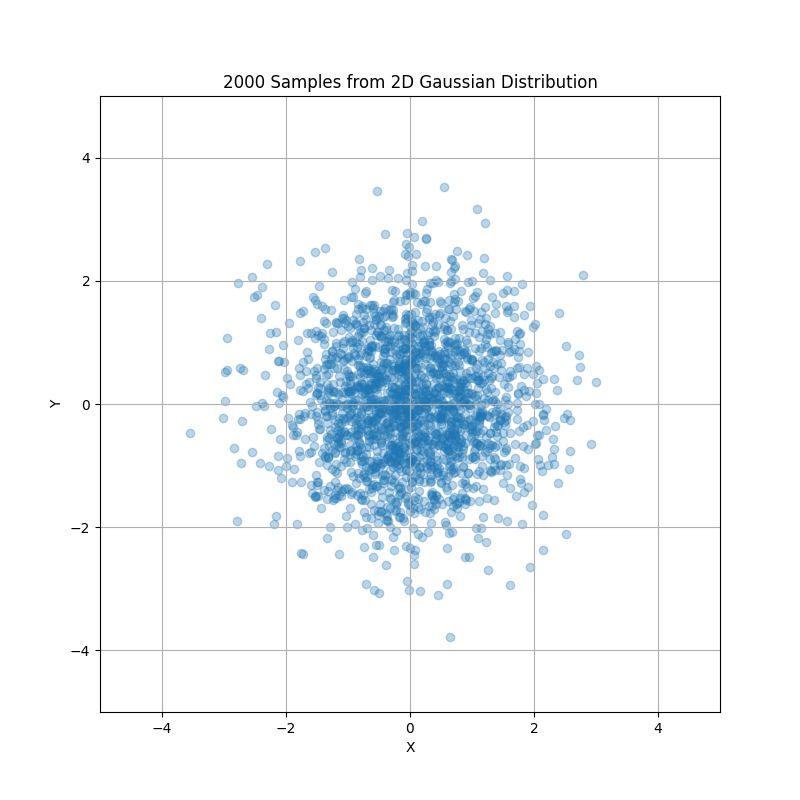
\includegraphics[width=\textwidth]{figures/gaussian_samples_2d.png}
                % \caption{Process 1}
            \end{figure}
        \end{column}
        \begin{column}{0.5\textwidth}
            \begin{figure}
                \centering
                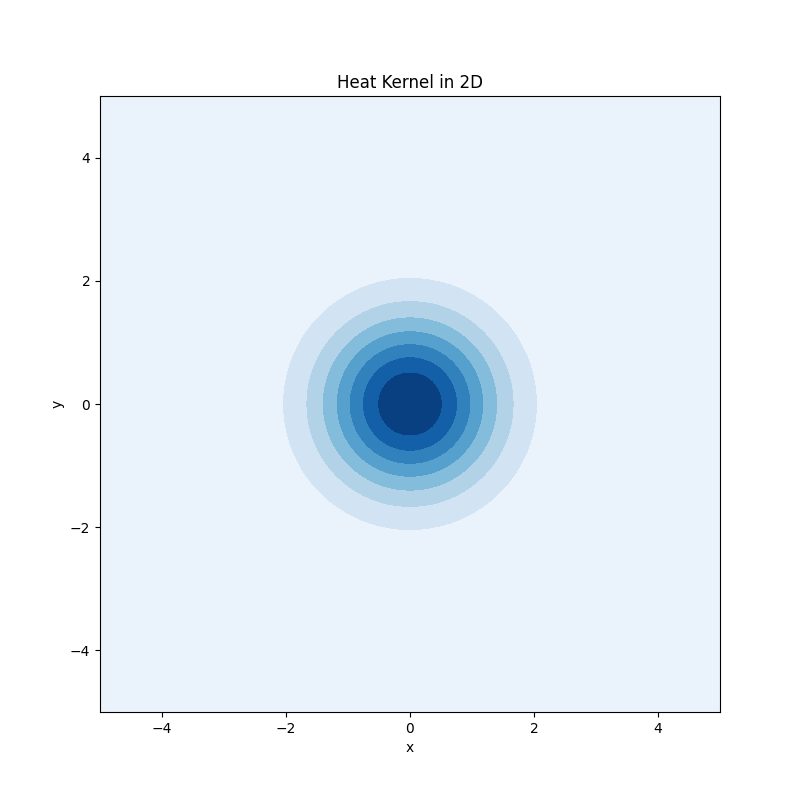
\includegraphics[width=\textwidth]{figures/heat_kernel_2d.png}
                % \caption{Process 2}
            \end{figure}
        \end{column}
    \end{columns}
\end{frame}

\section{Maximal Ergodic Theorem}

\begin{frame}{Maximal Ergodic Theorem}
    \begin{block}{Theorem. Maximal Ergodic Theorem}
        The harmonic extension of $f$, defined by $u(x, y) = P_y f(x)$, satisfies the following maximal inequality:

        \[
        \left\|\sup _{y>0} | u_f(\cdot, y)|\right\|_p \leq \frac{p}{p-1}\| f \|_p
        \]

        for all $f \in L^p$ and for all $1<p \leq \infty$. When $p=\infty$, we interpret the constant to be 1 .
    \end{block}
    \begin{block}{Proof scheme}
        \begin{enumerate}
            \item Construct a martingale $M_t$ from $X_t$, the process associated to the semigroup.
            \item Apply Doob's maximal inequality to $M_t$.
            \item Translate the inequality back to the semigroup.
        \end{enumerate}
    \end{block}

\end{frame}

\section{Martingales}

\begin{frame}{Martingales}
    \begin{itemize}
        \item \textbf{Probability Space}: A probability space is a measure space with total measure 1. Random variables are Borel-measurable functions.
        \item \textbf{Filtration}: A filtration is an increasing sequence of $\sigma$-algebras $\{\mathcal{F}_t\}_{t \geq 0}$ such that $\mathcal{F}_s \subseteq \mathcal{F}_t \subseteq \mathcal{F}$ for all $0 \leq s \leq t$.
        \item \textbf{Random Process}: A random process is an indexed collection of random variables $\{X_t\}_{t \geq 0}$.
    \end{itemize}

    \begin{block}{Martingale}
        A stochastic process $\{M_t\}_{t \geq 0}$ is a martingale with respect to a filtration $\{\mathcal{F}_t\}_{t \geq 0}$ if:
        \begin{itemize}
            \item $M_t$ is $\mathcal{F}_t$-measurable for all $t \geq 0$.
            \item $\mathbb{E}[|M_t|] < \infty$ for all $t \geq 0$.
            \item $\mathbb{E}[M_t \mid \mathcal{F}_s] = M_s$ for all $0 \leq s \leq t$.
        \end{itemize}
    \end{block}

    \begin{example}
        \begin{itemize}
            \item Winnings in a fair game.
            \item Brownian motion.
        \end{itemize}
    \end{example}
\end{frame}

% martingales cont.
\begin{frame}{Martingales, cont.}
    \begin{block}{Theorem. Doob's Maximal Inequality}
        Let $\{X_t\}_{t \geq 0}$ be a martingale. Then for all $p > 1$,
        \begin{equation*}
            \left\|\sup_{0 < t < T} |X_t^+|\right\|_p \leq \frac{p}{p-1} \left\|X_T^+\right\|_p
        .\end{equation*}
    \end{block}

    % burkholder-davis-gundy inequality
    \begin{block}{Theorem. Burkholder-Davis-Gundy Inequality, particular case}
        Let $\{M_t\}_{t \geq 0}$ be a martingale defined by the transform
        \begin{equation*}
            M_t = \int_0^t f(s,B_s) \, dB_s
        .\end{equation*}
        Then for all $p > 1$,
        \begin{equation*}
            \left\|M_t\right\|_p \leq C_p \left\|\left(\int_0^t |f(s, B_s)|^2 ds \right)^{1/2}\right\|_p
        \end{equation*}
        where $C_p$ is a constant depending only on $p$.
    \end{block}

    
\end{frame}

\section{Proof of Maximal Ergodic Theorem}

\begin{frame}{Proof of Maximal Ergodic Theorem}

    \begin{block}{Step 1}
        Let $X_t$ be the process associated to the Feller semigroup. Pick $T > 0$. Then $Q_{T - t} f(X_t)$ is a martingale.
    \end{block}
    Why? Because
    \begin{equation*}
        Q_{T - t} f(X_t) = \mathbb{E}^{X_t}[f(X_{T - t})] = \mathbb{E}^x [f(X_T) \mid \mathcal{F}_t]
    \end{equation*}
    \begin{exampleblock}{Intuition}
        A picture goes here.
    \end{exampleblock}
    
    
\end{frame}

\begin{frame}%{Proof of Maximal Ergodic Theorem, cont.}
    \begin{block}{Step 2}
        Apply Doob's maximal inequality to $Q_{T - t} f(X_t)$. We have
        \begin{equation*}
            E^x\left[\left(\sup_{0 < t < T} |Q_{T - t} f^+(X_t)|\right)^p\right]
            \leq \left(\frac{p}{p-1}\right)^p E^x\left[|f^+(X_T)|^p\right]
        \end{equation*}
    \end{block}
    \begin{exampleblock}{Intuition}
        A picture goes here. %TODO
    \end{exampleblock}

\end{frame}

\begin{frame}
    \begin{block}{Step 3}
        Integrate the right-hand side of the inequality. We have
        \begin{align*}
            \int E^x\left[ f^+(X_T)^p \right] \, dx 
            &= \int Q_T (|f^+|^p)(x) dx \\
            &= \left\langle Q_T(|f^+|^p), 1 \right\rangle \\
            &= \left\langle |f^+|^p, Q_T 1 \right\rangle & \text{self-adjointness of $Q_T$}\\
            &= \left\langle |f^+|^p, 1 \right\rangle & \text{identity preserving}\\
            &= \int |f^+(x)|^p \, dx \\
            &\leq \|f\|_p^p
        .\end{align*}
    \end{block}
    Thus
        \begin{equation*}
            \int E^x\left[ f^+(X_T)^p \right] \, dx \leq \|f\|_p^p
        \end{equation*}
\end{frame}

\begin{frame}
    \begin{block}{Step 3, cont.}
        Then consider the left-hand side. Want to show
        \begin{equation*}
            \mathbb{E}\left[\left(\sup_{0 < t < T} |Q_{T - t} f^+(X_t)|\right)^p\right]
            \only<-7>{\,\gtrsim \, \left\|\sup _{y>0} | u_f(\cdot, y)|\right\|_p^p}
        .\end{equation*}
    \end{block}
    \underline{Strategy}: Condition on $\mathcal{F}_T$ and turn into $f(X_T)$.

    \begin{align*}
        \mathbb{E}\left[\left(\sup_{0 < t < T} |Q_{T - t} f^+(X_t)|\right)^p\right]
        &= \mathbb{E}\left[E^x\left[\left(\sup_{0 < t < T} Q_{T - t} f^+(X_t)\right)^p \mid \mathcal{F}_T\right]\right] \\
        %
        \only<2-3>{&\geq \mathbb{E}\left[\sup_{0 < t < T} E^x\left[Q_{T - t} f^+({\only<3>{\color{red}}X_t}) \mid {\only<3>{\color{red}} \mathcal{F}_T}\right]^p \right] \\}
        %
        %
        \only<4->{&= \mathbb{E}\left[{\only<5>{\color{blue}}E^x}\left[\left(\sup_{0 < t < T} Q_{T - t} f^+(X_{\only<4>{\color{blue}} 2T - t})\right)^p \mid \mathcal{F}_T\right]\right] \\}
        %
        \only<5->{&\geq \mathbb{E}\left[\sup_{0 < t < T} {\only<5>{\color{blue}}E^x}\left[Q_{T - t} f^+(X_{2 T - t}) \mid {\only<6->{\color{olive}}\mathcal{F}_T}\right]^p \right] \\}
        \only<6->{&= \mathbb{E}\left[\sup_{0 < t < T} E^{{\only<6->{\color{olive}}X_T}}\left[Q_{T - t} f^+(X_{\only<6->{\color{blue}}T - t}) \right]^p \right] \\}
        \only<7->{&= \mathbb{E}\left[\sup_{0 < t < T} (Q_{\only<7>{\color{blue}}T - t} Q_{T - t} f^+({\color{olive}X_T}))^p \right] \\}
    \end{align*}
\end{frame}

\begin{frame}
    \begin{block}{Step 3, cont.}
        We have shown
        \begin{equation*}
            \mathbb{E}\left[\left(\sup_{0 < t < T} |Q_{T - t} f^+(X_t)|\right)^p\right]
            \,\geq \, \left\|\sup _{0 < t < T} | u_f(\cdot, 2t)|\right\|_p^p
        .\end{equation*}
    \end{block}
    Take $ T \to \infty$ on boths sides and we are done.

\end{frame}

\section{Fractional Integration and HLS Inequality}
\begin{frame}{Fractional Integration via Martingales}
    General strategy:
    \begin{enumerate}
        \item Give martingale representation of fractional integral.
        \item Apply martingale inequalities (Doob's and BDG).
    \end{enumerate} 
    \begin{block}{Theorem. [Applebaum and Ba\~nuelos, 2015] HLS for Heat Semigroup}
        For $f, a$ and $\alpha$ as above, we define for all $x \in \mathbb{R}^d$,
        \[
        \mathcal{S}^{a, \alpha} f(x)={E}\left(\int_0^a(a-s)^{\alpha / 2} \nabla\left(T_{a-s} f\right)\left(B_s\right) \cdot d B_s \mid B_a=x\right) .
        \]
        Then, for all $f \in \mathcal{S}\left(\mathbb{R}^d\right), x \in \mathbb{R}^d$
        \[
        \mathcal{S}^{a, \alpha} f(x)=-\int_0^a s^{\alpha / 2} T_s\left(\Delta T_s f\right)(x) d s
        \]
        and as $a \rightarrow \infty$,
        \[
        \mathcal{S}^{a, \alpha} f(x) \rightarrow I_\alpha(f)(x) .
        \]
        almost everywhere.
    \end{block}
\end{frame}

\begin{frame}{Step 1. Martingale representation}
    \begin{block}{Want to show}
       \[
        \mathcal{S}^{a, \alpha} f(x)
        \equiv E\left(\int_0^a(a-s)^{\alpha / 2} \nabla\left(T_{a-s} f\right)\left(B_s\right) \cdot d B_s \mid B_a=x\right)
        =-\int_0^a s^{\alpha / 2} T_s\left(\Delta T_s f\right)(x) d s
        \] 
    \end{block}
    \begin{align*}
        \int_{\mathbb{R}^d} \mathcal{S}^{a, \alpha} f(x) g(x) d x 
        &= \mathbb{E}\left( E\left(\int_0^a(a-s)^{\alpha / 2} \nabla\left(T_{a-s} f\right)\left(B_s\right) \cdot d B_s \mid B_a\right) g(B_a)\right) \\
        &= \mathbb{E}\left(\int_0^a(a-s)^{\alpha / 2} \nabla\left(T_{a-s} f\right)\left(B_s\right) \cdot d B_s g(B_a)\right) \\
        &=_{IF} \mathbb{E}\left(\int_0^a(a-s)^{\alpha / 2} \nabla\left(T_{a-s} f\right)\left(B_s\right)d B_s \, \int_0^a\nabla\left(T_{a-s} g\right)\left(B_s\right)d B_s\right)\\
        &=_{ISO} \mathbb{E}\left(\int_0^a(a-s)^{\alpha / 2} \nabla\left(T_{a-s} f\right)\left(B_s\right) \cdot \nabla\left(T_{a-s} g\right)\left(B_s\right) d s\right)\\
        &= \int_0^a s^{\alpha / 2}\int_{\mathbb{R}^d} \nabla\left(T_s f\right)(x) \cdot \nabla\left(T_s g\right)(x) d x d s \\
        &= - \int_{\mathbb{R}^d} \int_0^a s^{\alpha / 2} T_s \Delta T_{s} f(x) ds g(x) d x
    \end{align*}
\end{frame}

\begin{frame}{Step 2. Apply martingale inequalities}
    \begin{block}{Want to show}
        For $1/q = 1/p - \alpha/d$,
        \[
        \left\|\mathcal{S}^{a, \alpha} f\right\|_q \leq C_q \left\|f\right\|_p
        .\]
    \end{block}
    \begin{align}
        &\left\| \int_0^a (a - s)^{\alpha/2} \nabla(T_{a-s} f)(B_s) \cdot dB_s \right\|_q\\
        &\leq C_q \left\| \left( \int_0^a |(a - s)^{\alpha} \left| (\nabla T_{a-s} f)(B_s) \right|^2 ds \right)^{1/2} \right\|_q  & \text{by BDG} \\
        &\leq C_q \left\| C_{p, \alpha, d} \left( \sup_{0 < s < a} \left( T_{2 (a - s)}  |f| \right) (B_s) \right) ^{p / q} \right\|_q \|f\|_p^{\alpha p / d}
    \end{align}
    and apply Doob's maximal inequality to the supremum part.
\end{frame}

\begin{frame}{HLS for general semigroups}
    \begin{block}{Theorem. [Kim 2015]}
        Define
        \begin{equation*}
            \mathcal{T}_\alpha^s(f)(x) = E^s \left( \int_0^\tau Y_t^\alpha \frac{\partial u_f}{\partial y} (X_t, Y_t) d Y_t \mid X_\tau = x \right)
        \end{equation*}
        where $X_t$ is the process associated to the semigroup, $Y_t$ is a 1-d Brownian motion starting from $s$, and $\tau$ is time when $Y_t$ hits $0$.

        Then $\mathcal{T}_\alpha^s(f)(x)$ is the fractional integral just as in the last theorem, and the HLS inequality holds.
    \end{block}
    \begin{exampleblock}{Limitation}
        \begin{itemize}
            \item The proof for heat kernel is dependent on geometry of $\mathbb{R}^d$. This dependence is removed in the proof for general semigroups.
            \item However, the constant $C_q$ from probabilistic inequalities, though explicit, is not optimal. The optimal constant is attained by a different proof using symmetric decreasing rearrangement.
            \item It remains open whether one can obtain the optimal constant using probability theory.
        \end{itemize}
    \end{exampleblock}
\end{frame}


%% REFERENCES
\begin{frame}
    \begin{center}
        \Huge Questions?
    \end{center}
\vfill
    
\begin{itemize}
    \item
    David Applebaum and Rodrigo Bañuelos, \emph{Probabilistic Approach to Fractional Integrals and the Hardy-Littlewood-Sobolev Inequality}, in V. V. Mityushev and M. Ruzhansky (eds.), {Analytic Methods in Interdisciplinary Applications}, Vol. 116, Springer International Publishing, 2015, pp. 17--40. \url{https://doi.org/10.1007/978-3-319-12148-2_2}

    \item
    Doyoon Kim, \emph{Martingale transforms and the Hardy-Littlewood-Sobolev inequality for semigroups}, arXiv, 2015. \url{https://doi.org/10.48550/arXiv.1506.01208}

    \end{itemize}
\end{frame}
\end{document}
